\chapter{CMSIS}
CMSIS is a huge advantage in code portability. The idea behind that standardized
interface is to make the programmer independent of the hardware. Thus CMSIS is a
hardware abstraction layer.\\
The programmer develops code to access the CMSIS driver library instead of the
hardware. This way the code becomes portable for all CORTEX MCU's.
The following diagram gives an overview about CMSIS:\citep{ARM-CMSIS}\\

\begin{figure}[ht]
	\centering
	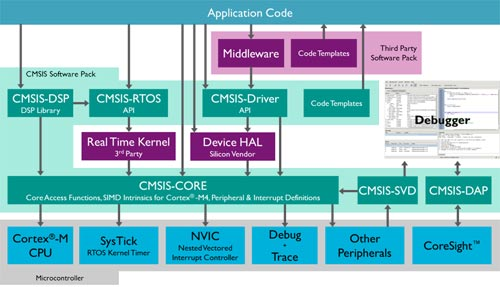
\includegraphics[width=420px, height=280px]{../img/cmsis.jpg}
	\caption{CORTEX MICROCONTROLLER SOFTWARE STANDARD INTERFACE}
	\label{cmsis_}
\end{figure}
